\documentclass[11pt]{article}

\usepackage[a4paper,margin=1.05in]{geometry}
\usepackage[utf8]{inputenc}
\usepackage{microtype}
\usepackage{amsmath,amssymb}
\usepackage{booktabs}
\usepackage{graphicx}
\usepackage{enumitem}
\usepackage{xcolor}
\usepackage{tikz}
\usetikzlibrary{positioning,arrows.meta}
\usepackage[labelfont=bf,font=small,labelsep=colon]{caption}
\usepackage[authoryear,round]{natbib}
\usepackage[colorlinks=true,linkcolor=blue!60!black,citecolor=blue!60!black,urlcolor=blue!60!black]{hyperref}
\usepackage[capitalise,noabbrev]{cleveref}

% Generated by make_figures.py. Do not edit.
\newcommand{\NTrain}{31\,157\,015}
\newcommand{\NTest}{20\,662\,282}
\newcommand{\NEval}{20\,659\,283}
\newcommand{\WinN}{3000}
\newcommand{\WinM}{3000}
\newcommand{\Thr}{251}
\newcommand{\Vocab}{182}
\newcommand{\NSize}{13}
\newcommand{\Corr}{0.56}
\newcommand{\CorrLo}{0.42}
\newcommand{\CorrHi}{0.60}
\newcommand{\CorrDay}{0.90}
\newcommand{\FlagShare}{7.6\%}
\newcommand{\MeanSurp}{3.22}
\newcommand{\MeanRar}{4.33}
\newcommand{\SurpFlag}{3.35}
\newcommand{\SurpRest}{3.21}
\newcommand{\SurpGap}{0.15}
\newcommand{\DecNine}{3.40}
\newcommand{\DecTen}{3.36}
\newcommand{\DecLow}{2.8}
\newcommand{\DecHigh}{3.4}
\newcommand{\DecTop}{3.4}
\newcommand{\GapLow}{1.2}
\newcommand{\GapHigh}{1.1}
\newcommand{\GapAvg}{1.1}
\newcommand{\RarCorr}{0.68}
\newcommand{\PrevCorr}{0.63}
\newcommand{\PrevMean}{3.51}
\newcommand{\ModCorr}{0.56}
\newcommand{\FieldSide}{$-$0.01}
\newcommand{\FieldSize}{0.58}
\newcommand{\FieldMove}{0.49}
\newcommand{\PrevShare}{73\%}
\newcommand{\LevelGain}{0.04}
\newcommand{\ModelGain}{1.11}
\newcommand{\LevelShare}{4\%}
\newcommand{\EntLow}{3.97}
\newcommand{\EntHigh}{4.41}
\newcommand{\BigCalm}{10\%}
\newcommand{\BigVol}{26\%}
\newcommand{\SeedBest}{2}
\newcommand{\SeedSpread}{0.0129}
\newcommand{\LossBest}{3.117}
\newcommand{\BlockLen}{1\,000\,000}
\newcommand{\NBoot}{2\,000}
\newcommand{\SEUsed}{0.045}
\newcommand{\Params}{2\,802\,816}
\newcommand{\Steps}{1901}
\newcommand{\TrainMinutes}{71}


\setlist{itemsep=2pt,topsep=4pt}
\newcommand{\RV}{\mathrm{RV}}
\newcommand{\nats}{\text{nats}}
\crefname{appendix}{Appendix}{Appendices}
\crefname{section}{Section}{Sections}

\title{A language model of the Bitcoin trade tape\\is surprised by volatility}
\author{Navid Nabijou\thanks{Queen Mary University of London. nn333@cantab.ac.uk}}
\date{October 10, 2026}

\begin{document}
\maketitle

\begin{abstract}
\noindent
We train a small causal transformer on a tokenised sequence of Bitcoin trades and ask whether its surprise tracks market volatility.
Each trade event becomes one token that records its side, its size and the price move it causes.
The model is trained on two months and scored on the following month, which holds approximately 20M events.
Its rolling mean surprisal correlates with realised volatility at \Corr{}.
A simple benchmark shows that part of this link is built in, because large price moves are rare tokens and also make up volatility.
The model is nevertheless far less surprised than a benchmark that scores each event only by how rare its token is.
It stays about \GapHigh{} nats below the benchmark even in the most volatile tenth of the month.
\end{abstract}

%% ------------------------------------------------------------------------------------
\section{Introduction}

Financial markets alternate between calm and turbulent regimes.
Large price changes tend to cluster in time \citep{cont2007}, and the level of activity moves between low and high states.
A model trained on the stream of trades could notice such a switch if it is surprised whenever the market departs from what it has learned.
Perplexity, the exponential of the mean surprisal, is the standard summary of how surprised a language model is.
We ask whether the perplexity of a transformer trained on the trade tape rises when the market is volatile.

We treat the tape as a language.
Each trade event becomes one token.
An event is one taker order, which is an order that executes immediately against orders already resting in the market.
The token records the side of the order, its size and the price move it causes.
No knowledge of finance is assumed, and \cref{app:data} explains the terms used.
The vocabulary has \Vocab{} tokens.
A small causal transformer is trained on two months of Bitcoin trades and then frozen.
We score every event of the following month by its surprisal.
We average the surprisal over windows of \WinN{} events and compare the average with realised volatility over the same events.

The question is one of detection.
We ask whether surprisal is high when volatility is high at the same time.
We do not ask whether surprisal predicts later volatility.

The findings fall into two parts.
\begin{enumerate}
  \item \textbf{The model is surprised by volatility.}
  Rolling mean surprisal and log realised volatility correlate at \Corr{} over \NEval{} test events, with a 95\% block-bootstrap interval of \CorrLo{} to \CorrHi{}.
  Surprisal is \SurpGap{} nats higher in the high-volatility regime than elsewhere (\cref{sec:surprised}).
  \item \textbf{But less surprised than rarity alone would suggest.}
  Part of this link is built in, because large price moves are rare tokens and also make up volatility.
  A benchmark that scores each event only by the rarity of its token averages \MeanRar{} nats per event, and the model averages \MeanSurp{}.
  The model stays about \GapHigh{} nats below the benchmark even in the most volatile tenth of the data (\cref{sec:rarity}).
\end{enumerate}

\Cref{sec:method} describes the design.
\Cref{sec:surprised,sec:rarity} give the two parts of the result.
\Cref{sec:discussion} offers labelled interpretation, \cref{sec:limits} states the limitations, and \cref{sec:related} reviews related work.
The appendices give the data, the tokeniser, the model, the statistics and the detailed results.

%% ------------------------------------------------------------------------------------
\section{Method}\label{sec:method}

\begin{figure}[t]
\centering
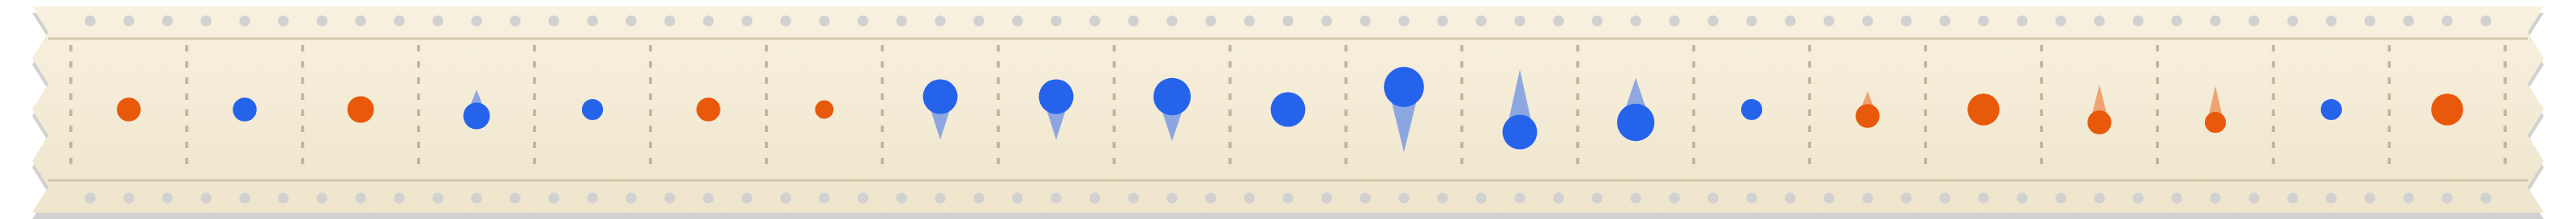
\includegraphics[width=\linewidth]{figures/tape.png}\\[6pt]
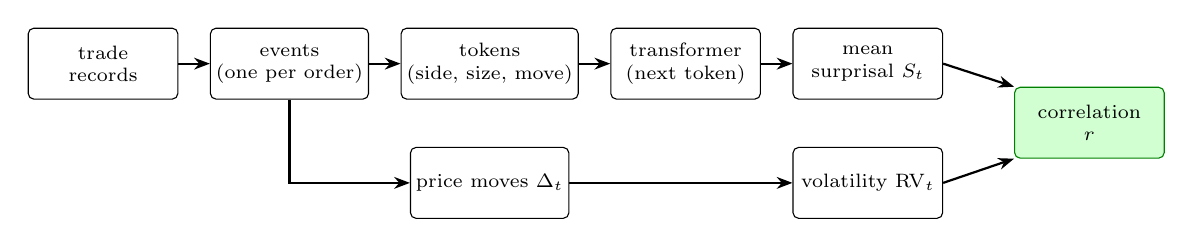
\begin{tikzpicture}[
  box/.style={draw,rounded corners=2pt,align=center,font=\scriptsize,minimum height=9mm,minimum width=19mm,inner sep=2pt},
  res/.style={box,fill=green!18,draw=green!50!black},
  arr/.style={-{Stealth[length=2mm]},thick},
  node distance=4mm]
  \node[box] (rec) {trade\\records};
  \node[box,right=of rec] (ev) {events\\(one per order)};
  \node[box,right=of ev] (tok) {tokens\\(side, size, move)};
  \node[box,right=of tok] (gpt) {transformer\\(next token)};
  \node[box,right=of gpt] (s) {mean\\surprisal $S_t$};
  \node[box,below=6mm of tok] (mv) {price moves $\Delta_t$};
  \node[box,below=6mm of s] (rv) {volatility $\RV_t$};
  \node[res,right=9mm of s,yshift=-7.5mm] (r) {correlation\\$r$};
  \draw[arr] (rec) -- (ev);
  \draw[arr] (ev) -- (tok);
  \draw[arr] (tok) -- (gpt);
  \draw[arr] (gpt) -- (s);
  \draw[arr] (ev) |- (mv);
  \draw[arr] (mv) -- (rv);
  \draw[arr] (s.east) -- (r.north west);
  \draw[arr] (rv.east) -- (r.south west);
\end{tikzpicture}
\caption{The design. Trade records are merged into events and each event becomes a token. A transformer trained on September and October scores each event of November by its surprisal. The rolling mean surprisal is compared with the realised volatility computed from the same events. The strip at the top shows a stretch of tokens: colour is the side, dot size is the trade size, and the tail is the price move.}
\label{fig:design}
\end{figure}

\subsection{Data and tokens}

The data are the aggregate trades of BTCUSDT on Binance spot \citep{binance}.
BTCUSDT is Bitcoin traded against USDT, a token pegged to the US dollar, and spot means immediate settlement.
\Cref{app:data} explains this and the other market terms we use.
We use 91 days from 1 September to 30 November 2025 (UTC).
September and October form the training period (61 days) and November is the test month (30 days).
The split is chronological.

A taker order that is large enough to sweep several price levels appears as several consecutive records.
We merge consecutive records into one event when they share the side and the timestamp, and the price continues in the aggressor's direction.
This gives 51.8 million events from 101.8 million records (\cref{app:data}).

Each event becomes one token with three fields.
\begin{itemize}
  \item \textbf{Side:} buy or sell, according to which party took the liquidity.
  \item \textbf{Size:} the quantity traded, binned on a logarithmic scale with three bins per decade and \NSize{} bins in total.
  \item \textbf{Price move:} the change in the last fill price from the previous event, in ticks of 0.01 USDT (the smallest price step).
  It falls into one of seven classes: flat, one tick up or down, and a mid or large move in each direction.
\end{itemize}
The vocabulary is $2\times\NSize\times 7=\Vocab{}$.
The tokens carry no timestamps (\cref{app:tokens}).

\Cref{fig:key} shows how we draw tokens.
Each token is a comet: the colour is the side, the radius of the dot is the size bin, and the tail records the price move.
The tail trails behind the dot, so a rising price puts the dot high with a tail below it, and a falling price does the opposite.
The strip at the top of \cref{fig:design} is a stretch of tokens drawn this way.

\begin{figure}[t]
\centering
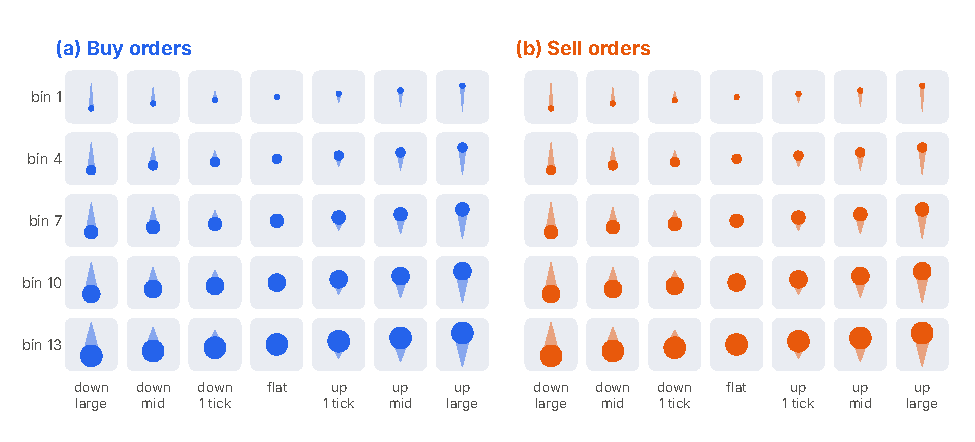
\includegraphics[width=\linewidth]{figures/token_key.pdf}
\caption{Key to the token icons, for a sample of five of the \NSize{} size bins. Columns are the seven price-move classes, from a large fall to a large rise. Rows are size bins from small to large, and the dot radius grows with the bin. Blue marks a buy and orange a sell.}
\label{fig:key}
\end{figure}

\subsection{Model and scoring}

The model is a decoder-only transformer \citep{vaswani2017,radford2019} with six layers, width 192, six attention heads, a context of 512 events and \Params{} parameters.
It is trained by next-token cross-entropy in a single pass over the training events.
We train three seeds with one recipe and keep the seed with the lowest final training loss.
The weights are then frozen, and no test data enter the choice (\cref{app:model}).

The surprisal of event $t$ is
\begin{equation}
  s_t = -\log p_\theta\!\left(x_t \mid x_{t-h},\dots,x_{t-1}\right),
\end{equation}
where the history length $h$ lies between 448 and 511 events for every scored event (\cref{app:scoring}).
The rolling mean over the last $N=\WinN{}$ events is $S_t=\frac1N\sum_{i=t-N+1}^{t}s_i$.

\subsection{Volatility and the statistic}

Realised volatility in event time is the root mean square of the price moves $\Delta_i$ over the last $M=\WinM{}$ events,
\begin{equation}
  \RV_t=\Bigl(\tfrac1M\sum_{i=t-M+1}^{t}\Delta_i^2\Bigr)^{1/2}.
\end{equation}
Because $N=M$, the two series summarise the same events.
The high-volatility regime is $\RV_t$ above the 90th percentile of the training period, which is \Thr{} ticks.
The regime flag is used for shading and for the comparison in \cref{sec:surprised}.
It does not enter the headline statistic.

The headline statistic is the Pearson correlation $r$ between $S_t$ and $\log\RV_t$ over the test month.
Both series are averages over overlapping windows, so neighbouring values are almost identical.
We therefore compute a 95\% interval by a moving-block bootstrap with blocks of \BlockLen{} events and \NBoot{} replicates (\cref{app:stats}).
All settings above were fixed before the model was scored.

%% ------------------------------------------------------------------------------------
\section{The model is surprised by volatility}\label{sec:surprised}

\begin{figure}[t]
\centering
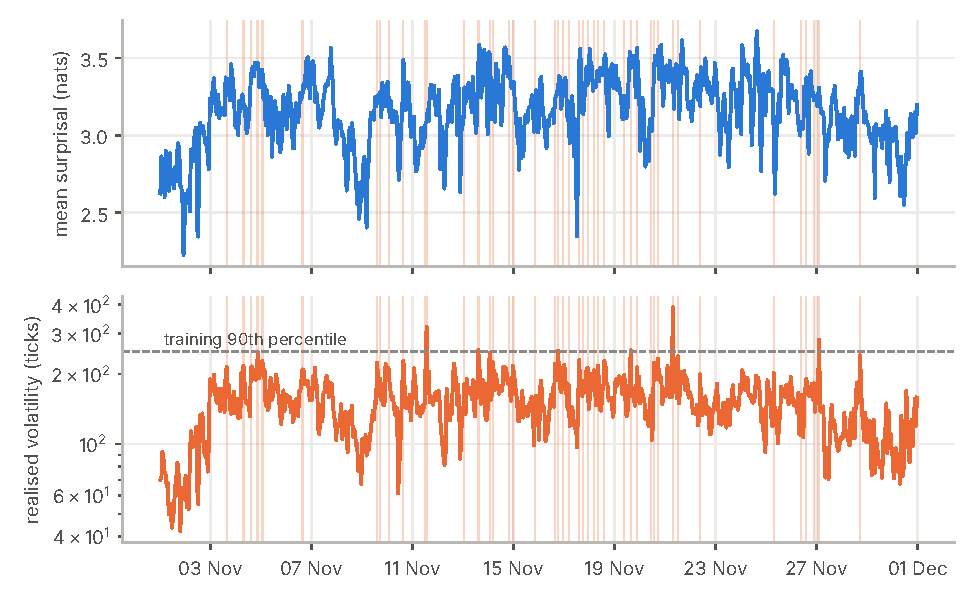
\includegraphics[width=\linewidth]{figures/series.pdf}
\caption{Hourly averages over the test month, November 2025. Top: mean surprisal. Bottom: realised volatility on a log scale, with the training 90th percentile dashed. Shading marks hours in which at least a fifth of the events exceed that threshold.}
\label{fig:series}
\end{figure}

\Cref{fig:series} shows the two series over the test month.
Surprisal and volatility rise and fall together.
The correlation is \Corr{} with a 95\% interval of \CorrLo{} to \CorrHi{}.

The regime comparison gives the same picture.
Mean surprisal is \SurpFlag{} nats where volatility is above the training threshold and \SurpRest{} nats elsewhere, a difference of \SurpGap{} nats.
\Cref{fig:relation}a groups the events by volatility decile.
Surprisal rises from \DecLow{} nats in the calmest decile to \DecNine{} in the ninth.
It then does not rise further, and it is \DecTen{} in the tenth.
The daily means of the 30 test days correlate at \CorrDay{} (\cref{fig:relation}b).
That figure is a description of 30 points and not a test.

\begin{figure}[t]
\centering
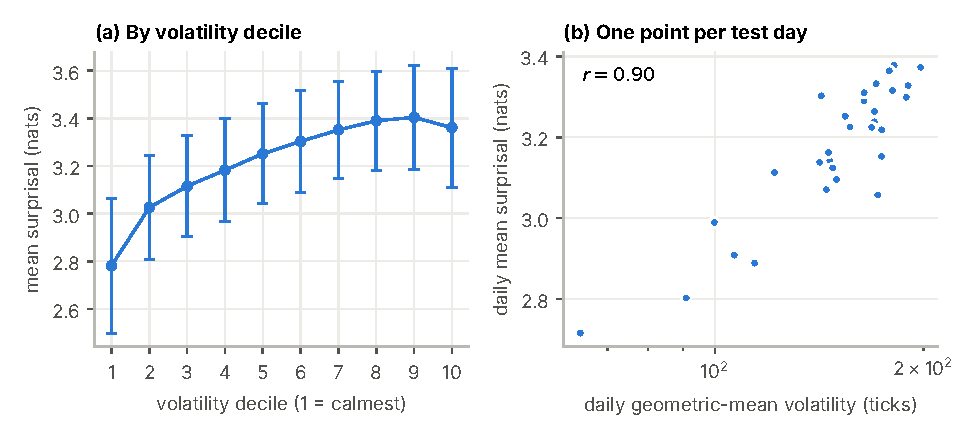
\includegraphics[width=\linewidth]{figures/relation.pdf}
\caption{(a) Mean surprisal by decile of realised volatility over the test month. Bars show one standard deviation of the rolling mean within the decile. (b) Daily means of surprisal against daily geometric-mean volatility.}
\label{fig:relation}
\end{figure}

We make no claim that surprisal leads volatility.
Shifting one series against the other lowers the correlation on both sides of zero (\cref{app:stats}).
That is expected from overlapping windows and carries no information about lead or lag.

%% ------------------------------------------------------------------------------------
\section{But less surprised than rarity alone would suggest}\label{sec:rarity}

To judge the model we need a reference.
Our reference is the rarity benchmark.
It scores each test event by the surprisal of its token under the token frequencies of the training period, with no context at all.

\textbf{The model is much less surprised than the benchmark.}
Averaged over the test month, the benchmark scores \MeanRar{} nats per event and the model scores \MeanSurp{} (\cref{fig:benchmark}a).
The gap is \GapLow{} nats in the calmest decile and \GapHigh{} nats in the most volatile one.
What the model learned from September and October therefore still applies when the market is volatile.

\begin{figure}[t]
\centering
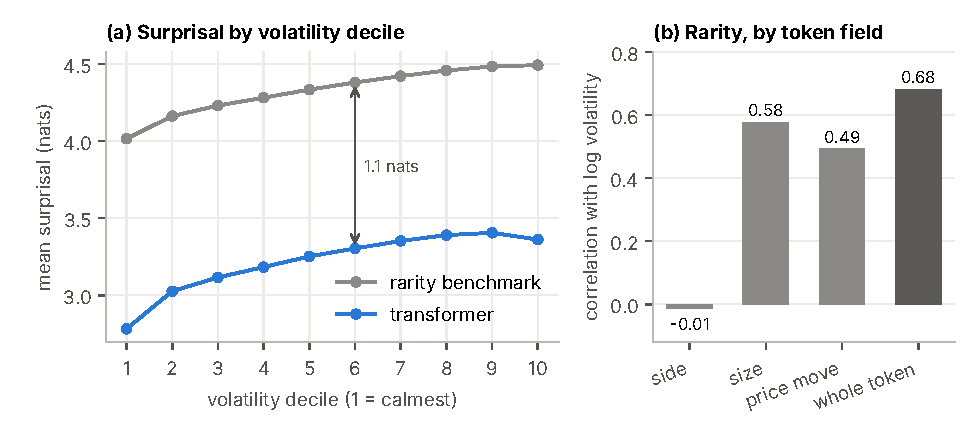
\includegraphics[width=\linewidth]{figures/benchmark.pdf}
\caption{(a) Mean surprisal by volatility decile for the rarity benchmark and the transformer. (b) Correlation with log volatility of the rolling mean rarity of each token field, and of the whole token.}
\label{fig:benchmark}
\end{figure}

\textbf{Part of the link in \cref{sec:surprised} is built in.}
Large price moves are rare tokens, and they are also what volatility is made of.
The rolling mean of the benchmark correlates with volatility at \RarCorr{}, above the model's \ModCorr{}.
The correlation of \cref{sec:surprised} therefore does not by itself show that the model has learned anything about sequences.
The decomposition in \cref{fig:benchmark}b shows where the link comes from.
It scores each field of the token separately.
\begin{itemize}
  \item \textbf{Price move:} the correlation is \FieldMove{}. This is expected by construction, because volatility is computed from price moves.
  \item \textbf{Size:} the correlation is \FieldSize{}. Size does not enter the volatility measure, so this part is market behaviour: trades are larger when the market is volatile.
  \item \textbf{Side:} there is no correlation (\FieldSide{}).
\end{itemize}
The contributions of size and price move overlap, because large trades often cause large moves, and they should not be added.

\textbf{Little of the model's gain comes from the volatility level.}
A model that knew only the volatility decile before each event would gain \LevelGain{} nats over the benchmark.
The transformer gains \ModelGain{} nats.
Knowing how volatile the market is therefore explains about \LevelShare{} of the improvement (\cref{app:rarity}).

%% ------------------------------------------------------------------------------------
\section{Discussion}\label{sec:discussion}

This section is interpretation.
We state it because it bears on how the results should be read.

\textbf{Why surprisal tracks volatility.}
A natural reading is that volatile markets are intrinsically less predictable.
In the test month the entropy of the token distribution, given the volatility decile before the event, rises from \EntLow{} to \EntHigh{} nats across the deciles (\cref{app:rarity}).
Even a model that knew the volatility level perfectly would be more surprised in volatile periods.
We have not tested this reading beyond that calculation.

\textbf{Why the top decile does not rise.}
The largest price-move class is open-ended above 129 ticks, about 1.29 USDT.
A very large move therefore falls in the same token as a moderately large one, and surprisal cannot grow once moves saturate.
We have not tested whether this explains the flattening.

\textbf{What the model has learned.}
Most of the model's gain over the benchmark is local.
The transformer gains \ModelGain{} nats over the benchmark.
A count-based model that sees only the previous token reaches \PrevShare{} of that gain (\cref{app:rarity}).
This model is a table of next-token frequencies given the previous token, estimated on the whole training period.
It is not a neural network.
The training loss of the transformer falls by about 0.14 nats as the history grows from a few events to several hundred (\cref{app:model}).
We do not claim that the model uses long context.

%% ------------------------------------------------------------------------------------
\section{Limitations}\label{sec:limits}

\textbf{One model, one month, one market.}
Only the selected seed was scored.
The final training losses of the three seeds differ by \SeedSpread{} nats, and the variation of the correlation across training runs is not measured.
The interval reflects resampling of the test month only.
The data are one asset on one venue over one month.
The test month is milder than the training period: \FlagShare{} of test events are in the high-volatility regime, against 10\% of training events, which is the definition of the threshold.

\textbf{Interval and windows.}
The interval depends on the block length.
The bootstrap standard error rises with block length and levels off near the length we used (\cref{app:stats}).
We did not vary $N$ or $M$.

\textbf{Tokenisation.}
We used one tokenisation and did not vary the bins.
The benchmark's rarity depends on the training mix of tokens.

\textbf{Scope.}
The result is simultaneous.
We do not test lead or lag, and we do not compare with standard volatility forecasting models such as GARCH, which predict volatility from past price changes.

%% ------------------------------------------------------------------------------------
\section{Related work}\label{sec:related}

Several works build generative models of order flow or of time series from tokens.
\begin{itemize}
  \item \citet{nagy2023} tokenise limit order book messages by digit groups and train a state-space model on them.
  \item \citet{linna2025} train a BERT-style model with one token per message.
  \item \citet{ansari2024} tokenise general time series by scaling and quantisation.
\end{itemize}
These works study generation or forecasting.
We did not find prior work that uses the surprisal of such a model as an indicator of the volatility regime.
Our search was not exhaustive.

The volatility measure is realised volatility \citep{andersen2003}, here computed in event time.
Event time is a transaction clock, and the cumulative number of trades is a better stochastic clock than volume for obtaining near-normal returns \citep{ane2000}.
Volatility clustering and the other stylised facts are reviewed by \citet{cont2001,cont2007}.
Trading volume is positively related to the size of price changes \citep{karpoff1987}, which is consistent with the link between trade size and volatility in \cref{sec:rarity}.
The moving-block bootstrap is due to \citet{kunsch1989}.
Automatic block-length rules exist \citep{politis2004,patton2009}, and we chose the length from the dependence of the series (\cref{app:stats}).

%% ------------------------------------------------------------------------------------
\section{Conclusion}

A small transformer trained on two months of Bitcoin trades is more surprised when the market is more volatile.
The correlation is \Corr{} on the test month, with a 95\% interval of \CorrLo{} to \CorrHi{}.
Part of that link is built in, because large moves are rare events and also make up volatility.
The model is nevertheless about \GapAvg{} nats less surprised than a benchmark that looks only at token rarity, and the margin holds in the most volatile decile.
Three follow-up studies would extend the result.
\begin{itemize}
  \item A lead test would ask whether surprisal rises before volatility does.
  \item Scoring the other seeds would measure the variation of the result across training runs.
  \item Other assets and months would test whether the result is specific to this market.
\end{itemize}

\section*{Acknowledgements}
Beyond the initial project design, this project's code, analysis and this write-up were developed in collaboration with Claude (Anthropic).

\bibliographystyle{plainnat}
\bibliography{refs}

%% ====================================================================================
\appendix

\section{Market terms and data}\label{app:data}

\paragraph{Market.}
A crypto exchange such as Binance runs a marketplace where people trade one asset for another.
BTCUSDT is the market in which Bitcoin (BTC) is bought and sold for USDT, a token whose value is pegged to the US dollar.
The price is the number of USDT per BTC.
A spot market settles trades immediately, as opposed to derivatives such as futures.

\paragraph{Order book, maker and taker.}
The exchange keeps an order book, a list of orders that are waiting to trade.
Each waiting order states a side (buy or sell), a price and a quantity, and is also called a limit order.
Buy orders are bids and sell orders are asks.
A trade happens when a new order meets a waiting order at an acceptable price.
\begin{itemize}
  \item A \emph{maker} order waits in the book and provides liquidity, meaning the chance for others to trade.
  \item A \emph{taker} order executes at once against waiting orders and removes liquidity.
  A market order is a taker order.
  \item The taker is the \emph{aggressor} of a trade.
  The side of a trade is the side of its taker.
  A buy taker consumes the lowest asks, which tends to raise the price, and a sell taker consumes the highest bids, which tends to lower it.
\end{itemize}

\paragraph{Sweeping.}
A waiting order has only a limited quantity.
A taker order larger than the quantity at the best price continues to the next price, and so on.
It is said to sweep several price levels.
The exchange reports the fill at each level as a separate trade, so one taker order can produce several records at the same instant and at steadily worse prices.

\paragraph{Aggregate trade records.}
Binance publishes aggregate trades, in which fills of one taker order at the same price are already combined.
Each record has the following fields.
\begin{itemize}
  \item An aggregate trade identifier that increases with time.
  \item A price and a quantity.
  \item A timestamp.
  \item A flag for whether the buyer was the maker.
  The aggressor is the seller when the buyer was the maker, and the buyer otherwise.
\end{itemize}

\paragraph{Units.}
A tick is the smallest price step, which is 0.01 USDT for BTCUSDT.
We write the price move of an event in ticks.
We count quantities in lots of $10^{-5}$ BTC.
Prices and quantities are held as integers in these units, so that no comparison involves rounding.

\paragraph{Volatility.}
Volatility measures how large the price changes are.
Realised volatility is computed from observed changes and not from a model.
We define it in event time in \cref{sec:method}.
Markets move between calm periods and volatile ones, which are called regimes, and large changes tend to cluster together.
We call a period a high-volatility regime when volatility is above a fixed threshold.

\paragraph{Source.}
The files are the daily \texttt{aggTrades} archives for BTCUSDT spot from \url{data.binance.vision} \citep{binance}.
Each file has a checksum, and every file was verified.
From 1 January 2025 the spot timestamps are in microseconds.

\paragraph{Cleaning.}
\begin{itemize}
  \item Records with zero price or zero quantity are audit duplicates and are dropped.
  \item Records are ordered by aggregate trade identifier.
\end{itemize}

\paragraph{Merging records into events.}
An event is one taker order.
A record joins the current event when it has the same side as the previous record, the same timestamp, and a price that continues strictly in the aggressor's direction.
Continuing means higher for a buy and lower for a sell.
Each day is processed on its own, and an order split by midnight within one microsecond would be cut in two, which is negligible.

\Cref{tab:merge} gives a worked example.
Four records give two events.
The first three records are one buy order that sweeps three prices.
The fourth record is a sell.

\begin{table}[h]
\centering\small
\begin{tabular}{rrrrcl}
\toprule
Record & Price & Quantity (BTC) & Timestamp & Side & Event \\
\midrule
1 & 82\,000.10 & 0.0020 & $t$   & buy  & 1 \\
2 & 82\,000.11 & 0.0150 & $t$   & buy  & 1 \\
3 & 82\,000.13 & 0.0400 & $t$   & buy  & 1 \\
4 & 82\,000.12 & 0.0010 & $t+1$ & sell & 2 \\
\bottomrule
\end{tabular}
\caption{Merging example. Event 1 has size 0.0570 BTC and last price 82\,000.13. Its price move is measured against the last price of the previous event.}
\label{tab:merge}
\end{table}

\paragraph{Counts.}
The 91 files hold 101{,}818{,}559 records, which merge into 51{,}819{,}298 events (1.96 records per event).
The first event has no previous price and is dropped.
This leaves \NTrain{} training events and \NTest{} test events.

%% ------------------------------------------------------------------------------------
\section{Tokeniser}\label{app:tokens}

\paragraph{Fields.}
A token is $(\text{side},\text{size},\text{move})$, coded as
\begin{equation}
  \text{id}=(\text{side}\cdot n_{\text{size}}+\text{size})\cdot 7+\text{move},
\end{equation}
with side 0 for sell and 1 for buy, size from 0 to $n_{\text{size}}-1$ and move from 0 to 6.
With $n_{\text{size}}=\NSize{}$ the vocabulary is \Vocab{}.

\paragraph{Price move.}
The move is the change in the last fill price of the event from the last fill price of the previous event, in ticks.
\Cref{tab:vocab} (left) lists the seven classes.
A move of 2 ticks or more is mid or large.
It is large when it exceeds 129 ticks, which is the median of such moves in the training period, and mid otherwise.
The boundaries are fitted on the training period only.

\paragraph{Size.}
Sizes are binned on a logarithmic scale with edges at $5\times 10^{k/3}$ lots for $k=1,\dots,15$, which is three bins per decade.
The tail rule merges an outer bin that holds less than 1\% of the training events into its inner neighbour, and repeats until the outermost bin holds at least 1\%.
This reduces the 16 raw bins to \NSize{}.
\Cref{tab:vocab} (right) lists the final bins.

\begin{table}[h]
\centering\small
\begin{minipage}[t]{0.42\linewidth}\centering\begin{tabular}{lr}
\toprule
Price move & Share of training events \\
\midrule
down, large & 4.3\% \\
down, mid & 4.4\% \\
down, 1 tick & 14.3\% \\
flat & 54.3\% \\
up, 1 tick & 14.4\% \\
up, mid & 4.1\% \\
up, large & 4.2\% \\
\bottomrule
\end{tabular}
\end{minipage}
\hfill
\begin{minipage}[t]{0.52\linewidth}\centering\begin{tabular}{rrr}
\toprule
Bin & Size range (BTC) & Share of training events \\
\midrule
1 & below 0.00011 & 13.1\% \\
2 & 0.00011--0.00023 & 9.4\% \\
3 & 0.00023--0.0005 & 9.5\% \\
4 & 0.0005--0.0011 & 12.5\% \\
5 & 0.0011--0.0023 & 10.2\% \\
6 & 0.0023--0.005 & 9.9\% \\
7 & 0.005--0.011 & 9.9\% \\
8 & 0.011--0.023 & 8.8\% \\
9 & 0.023--0.05 & 6.2\% \\
10 & 0.05--0.11 & 5.1\% \\
11 & 0.11--0.23 & 2.7\% \\
12 & 0.23--0.5 & 1.6\% \\
13 & above 0.5 & 1.2\% \\
\bottomrule
\end{tabular}
\end{minipage}
\caption{Left: the seven price-move classes and their shares of training events. Right: the size bins and their shares.}
\label{tab:vocab}
\end{table}

\paragraph{Icons.}
\Cref{fig:key} and the strip in \cref{fig:design} draw each token as a dot with a tail.
Colour is the side and dot radius is the size bin.
The tail points against the move, and its length is 4, 8 or 14 units on a 32-unit tile for a move of one tick, a mid move or a large move.
The tail extends that distance beyond the edge of the dot, whatever the size of the dot.

%% ------------------------------------------------------------------------------------
\section{Model and training}\label{app:model}

\paragraph{Architecture.}
The model is a decoder-only transformer with pre-normalisation \citep{xiong2020}, GELU activations \citep{hendrycks2016} and learned absolute position embeddings.
The input and output embeddings are tied \citep{press2017}.
There is no dropout.
\Cref{tab:hyper} lists the settings.

\begin{table}[h]
\centering\small
\begin{tabular}{ll}
\toprule
Setting & Value \\
\midrule
Layers, width, heads & 6, 192, 6 \\
Context & 512 events \\
Vocabulary & \Vocab{} \\
Parameters & \Params{} \\
Optimiser & AdamW \citep{loshchilov2019}, $\beta=(0.9,0.95)$ \\
Peak learning rate & $10^{-3}$, 100 warm-up steps, cosine decay to 10\% \\
Weight decay & 0.1, on weight matrices and embeddings only \\
Gradient clipping & 1.0 \\
Batch & 32 chunks of 512 events (16\,384 tokens) \\
Training & one pass, \Steps{} steps, chunks shuffled \\
Seeds & 0, 1, 2 \\
Software & PyTorch \citep{paszke2019} \\
\bottomrule
\end{tabular}
\caption{Model and training settings.}
\label{tab:hyper}
\end{table}

\paragraph{Training data.}
The training stream is cut into non-overlapping chunks of 512 events, giving 60{,}853 chunks, and the chunks are shuffled with a fixed seed.
The input is 512 consecutive events and the target is the same events shifted by one.
The last partial batch of 21 chunks is dropped, so the final 10{,}752 events of the training period are not used as targets.
The single pass means that every batch is new data, and there is no separate validation set.

\paragraph{Seed choice.}
\Cref{tab:seeds} gives the final training loss of each seed, the mean over the last tenth of the steps.
Seed \SeedBest{} has the lowest loss and is kept.
The choice uses training loss only.
\Cref{fig:training}a shows the three loss curves, which are almost indistinguishable.

\begin{table}[h]
\centering\small
\begin{tabular}{rrrr}
\toprule
Seed & Final training loss (nats) & Training time (min) & Selected \\
\midrule
0 & 3.1227 & 68 &  \\
1 & 3.1295 & 73 &  \\
2 & 3.1166 & 73 & yes \\
\bottomrule
\end{tabular}

\caption{Final training loss by seed. The spread is \SeedSpread{} nats. The runs were on a laptop CPU with four cores and no GPU.}
\label{tab:seeds}
\end{table}

\paragraph{Loss by position.}
\Cref{fig:training}b shows the mean training loss at each position within a chunk, averaged over the whole pass, so it includes the early steps.
The loss falls from about 3.34 nats after a few events of history to about 3.20 nats after a few hundred.
Scored events have between 448 and 511 events of history and so lie on the flat part.

\begin{figure}[h]
\centering
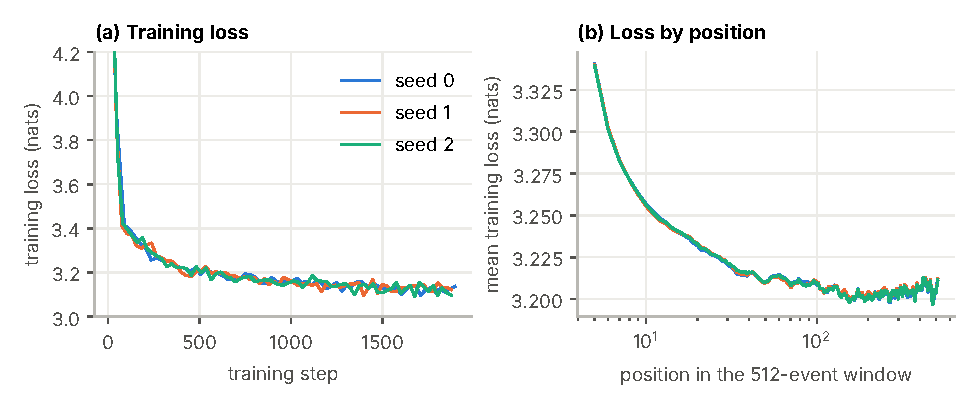
\includegraphics[width=\linewidth]{figures/training.pdf}
\caption{(a) Training loss of the three seeds, each point is the mean of the last 20 steps, sampled about once a minute. (b) Mean training loss by position in the 512-event chunk, smoothed over 8 positions, with a log axis.}
\label{fig:training}
\end{figure}

%% ------------------------------------------------------------------------------------
\section{Scoring}\label{app:scoring}

The model reads at most 512 events.
If the test stream were cut into plain chunks of 512, the first event of a chunk would have no history and the last would have 511.
Surprisal falls as history grows, so the series would show a spurious sawtooth.

Instead, a window of 512 events slides over the stream with a stride of 64 events, and only the last 64 events of each window are scored.
Let the extended stream be the last 511 training events followed by the test events.
The training events are context only and are never scored.
Test event $j$ (counting from 0) is scored in window $k=\lfloor j/64\rfloor$.
It is predicted from $448+(j \bmod 64)$ events of history, which lies between 448 and 511.
The test month has 322{,}849 windows.
A stride of 1 would give every event 511 events of history, but it would take about 5.5 days on our laptop, against about two hours for a stride of 64.

The implementation is checked against a brute-force computation of $-\log p$ for individual events, and a scoring run that is stopped and resumed gives the same result as an uninterrupted run.

%% ------------------------------------------------------------------------------------
\section{Volatility and the regime flag}\label{app:vol}

Realised volatility is computed on the continuous stream of training and test events.
A window near the start of the test month reaches back into the end of the training period, and uses only events that precede the one measured.
The regime flag is $\RV_t$ above the 90th percentile of $\RV_t$ over the training events with a full window, which is \Thr{} ticks.
It flags 10.0\% of training events and \FlagShare{} of test events.
The window $M=\WinM{}$ was chosen on 23 training days, before any test data were scored.
It balances noise from single large sweeps against resolution in time.
In the headline statistic $\RV_t$ is floored at $10^{-3}$ ticks before the logarithm.

%% ------------------------------------------------------------------------------------
\section{Statistics}\label{app:stats}

\paragraph{Moving-block bootstrap.}
Let $(x_t,y_t)_{t=1}^n$ be the series of $S_t$ and $\log\RV_t$ over the test month, with $n=\NEval{}$.
With block length $b$, the blocks are all windows of $b$ consecutive pairs.
A replicate has three steps.
\begin{enumerate}
  \item Draw $\lceil n/b\rceil$ block starts uniformly with replacement.
  \item Glue the blocks and cut the result to length $n$.
  \item Recompute the correlation.
\end{enumerate}
We use $b=\BlockLen{}$ and \NBoot{} replicates.
The interval is the 2.5th and 97.5th percentiles of the replicates \citep{kunsch1989}.
Each replicate needs only the five sums $\sum x$, $\sum y$, $\sum x^2$, $\sum y^2$ and $\sum xy$ over its blocks.
These are differences of prefix sums, evaluated at the few thousand positions that are needed, so \NBoot{} replicates over \NEval{} events run in seconds.

\paragraph{Block length.}
The length $b=\BlockLen{}$ is about one and a half days of the test month, which gives about 21 blocks.
It was fixed before scoring from the autocorrelation of $\log\RV$ in the training period.
\Cref{fig:checks}a and \cref{tab:blocks} (left) show the bootstrap standard error as a function of block length on the test series.
The error rises with block length and levels off near the length used, at \SEUsed{}.
Automatic rules for the block length exist \citep{politis2004,patton2009}, and we did not use them.
\Cref{tab:blocks} (right) gives the autocorrelation of the two series.

\begin{table}[h]
\centering\small
\begin{minipage}[t]{0.50\linewidth}\centering\begin{tabular}{rrr}
\toprule
Block length & Std. error & 95\% interval \\
\midrule
1\,000 & 0.007 & [0.54\, 0.57] \\
10\,000 & 0.017 & [0.52\, 0.59] \\
100\,000 & 0.030 & [0.49\, 0.61] \\
300\,000 & 0.040 & [0.46\, 0.62] \\
1\,000\,000 & 0.045 & [0.42\, 0.60] \\
2\,000\,000 & 0.041 & [0.41\, 0.57] \\
\bottomrule
\end{tabular}
\end{minipage}
\hfill
\begin{minipage}[t]{0.42\linewidth}\centering\begin{tabular}{rrr}
\toprule
Lag & $\log\mathrm{RV}$ & Surprisal \\
\midrule
3\,000 & 0.67 & 0.74 \\
30\,000 & 0.46 & 0.48 \\
300\,000 & 0.16 & 0.15 \\
1\,000\,000 & 0.05 & 0.06 \\
\bottomrule
\end{tabular}
\end{minipage}
\caption{Left: bootstrap standard error and 95\% interval of the correlation by block length. Right: autocorrelation of $\log\RV$ and of the mean surprisal.}
\label{tab:blocks}
\end{table}

\paragraph{Shifted series.}
\Cref{fig:checks}b recomputes the correlation after shifting the surprisal series against the volatility series.
It is highest at zero shift and falls on both sides.
Windows overlap, so a shift of less than $N$ events keeps most of the window in common.
The figure is not a lead test.

\begin{figure}[h]
\centering
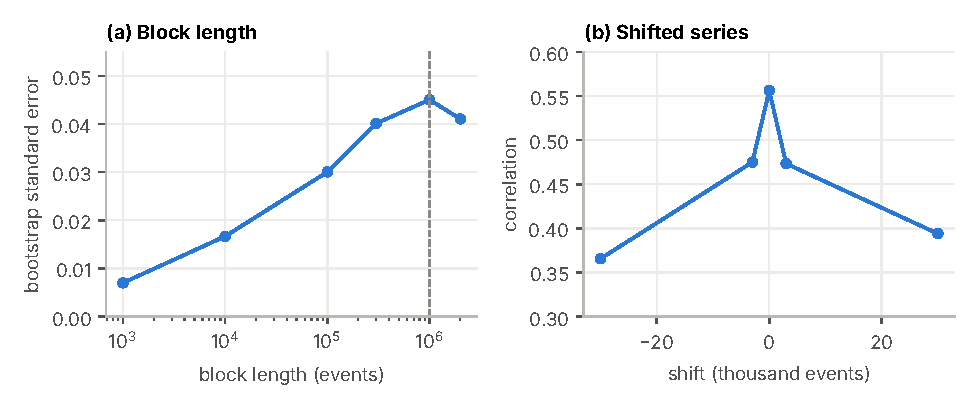
\includegraphics[width=\linewidth]{figures/checks.pdf}
\caption{(a) Bootstrap standard error of the correlation by block length. The dashed line marks the length used. (b) Correlation after shifting the surprisal series by the given number of events.}
\label{fig:checks}
\end{figure}

%% ------------------------------------------------------------------------------------
\section{Rarity benchmark and further results}\label{app:rarity}

\paragraph{Definition.}
Let $c_v$ be the count of token $v$ in the training stream, with 0.5 added to every count.
The rarity of a token is $-\log\bigl(c_v/\sum_u c_u\bigr)$.
The rarity benchmark scores each test event by the rarity of its token.
Its rolling mean over $N$ events is compared with volatility exactly as the model's is.
The benchmark uses the training period only.

\paragraph{Ladder of scoring rules.}
\Cref{tab:ladder} adds a model that sees only the previous token.
It is a table of next-token frequencies given the previous token, counted over the whole training period, and it is not a neural network.
The counts are smoothed towards the token frequencies, by adding $\alpha\times\Vocab{}$ pseudo-counts spread according to those frequencies.
We chose $\alpha=\PrevAlpha{}$ by fitting the counts on the first 85\% of the training period and scoring the last 15\%, and then refitted the counts on all of it.
On the held-out part, any $\alpha$ between 0.1 and 2 gives a mean surprisal within 0.001 nats of the best.
The slope is the change of the rolling mean surprisal in nats per unit of $\log\RV$.
Better models are less surprised on average.
Their correlation with volatility is lower.
Their slopes are not lower, so the lower correlation comes from more spread in the surprisal that is unrelated to volatility.

\begin{table}[h]
\centering\small
\begin{tabular}{lrrrr}
\toprule
Scoring rule & Mean surprisal & Correlation & Slope & Flagged minus rest \\
 & (nats) & with $\log\mathrm{RV}$ & (nats per unit) & (nats) \\
\midrule
Token rarity (no context) & 4.33 & 0.68 & 0.35 & 0.18 \\
Previous token only & 3.51 & 0.63 & 0.45 & 0.21 \\
Transformer (512 events) & 3.22 & 0.56 & 0.42 & 0.15 \\
\bottomrule
\end{tabular}

\caption{Three scoring rules on the test month. ``Flagged minus rest'' is the difference in mean rolling surprisal between flagged and unflagged events.}
\label{tab:ladder}
\end{table}

\paragraph{By volatility decile.}
\Cref{tab:deciles} gives the numbers behind \cref{fig:benchmark}a.
\Cref{fig:level} adds a model that knows only the volatility decile before each event.
Its score is the empirical entropy, in nats, of the token distribution among events whose preceding volatility lies in the decile, computed on the test month.
The entropy rises from \EntLow{} nats in the calmest decile to \EntHigh{} in the most volatile.

\begin{table}[h]
\centering\small
\begin{tabular}{rrrrr}
\toprule
Decile & RV range (ticks) & Transformer & Rarity & Gap \\
\midrule
1 & 15--103 & 2.78 & 4.02 & 1.23 \\
2 & 103--123 & 3.03 & 4.16 & 1.14 \\
3 & 123--138 & 3.12 & 4.23 & 1.11 \\
4 & 138--150 & 3.18 & 4.28 & 1.10 \\
5 & 150--162 & 3.25 & 4.33 & 1.08 \\
6 & 162--174 & 3.30 & 4.38 & 1.08 \\
7 & 174--187 & 3.35 & 4.42 & 1.07 \\
8 & 187--204 & 3.39 & 4.46 & 1.07 \\
9 & 204--236 & 3.40 & 4.48 & 1.08 \\
10 & 236--3258 & 3.36 & 4.49 & 1.13 \\
\bottomrule
\end{tabular}

\caption{Mean surprisal in nats by volatility decile (deciles of the rolling window volatility $\RV$). ``Gap'' is rarity minus transformer.}
\label{tab:deciles}
\end{table}

\begin{figure}[h]
\centering
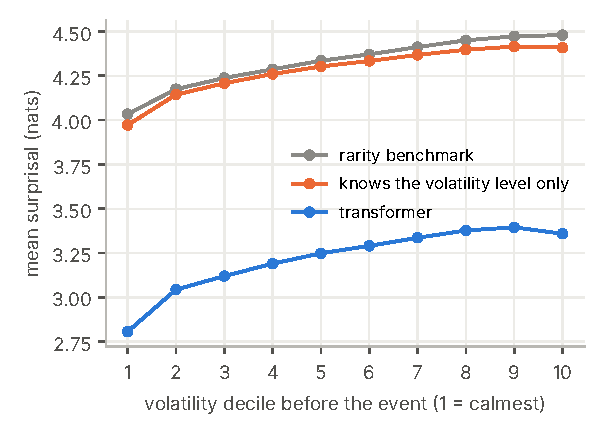
\includegraphics[width=0.62\linewidth]{figures/level_only.pdf}
\caption{Mean surprisal by the volatility decile before the event. A model that knew only the volatility decile gains little over the rarity benchmark.}
\label{fig:level}
\end{figure}

\paragraph{Token fields.}
\Cref{tab:fields} gives the correlations behind \cref{fig:benchmark}b.
In the calmest decile \BigCalm{} of events have a mid or large move.
In the most volatile decile the share is \BigVol{}.

\begin{table}[h]
\centering\small
\begin{tabular}{lr}
\toprule
Rarity of the token's \ldots & Correlation with $\log\mathrm{RV}$ \\
\midrule
side & $-$0.01 \\
price move & 0.49 \\
trade size & 0.58 \\
whole token & 0.68 \\
\bottomrule
\end{tabular}

\caption{Correlation with $\log\RV$ of the rolling mean rarity of each field of the token.}
\label{tab:fields}
\end{table}

\paragraph{By token class.}
\Cref{fig:classes} gives the mean surprisal for each price-move class and each size bin.
The model is below the benchmark in every class.
Flat moves are the least surprising, and large trades are the most surprising.

\begin{figure}[h]
\centering
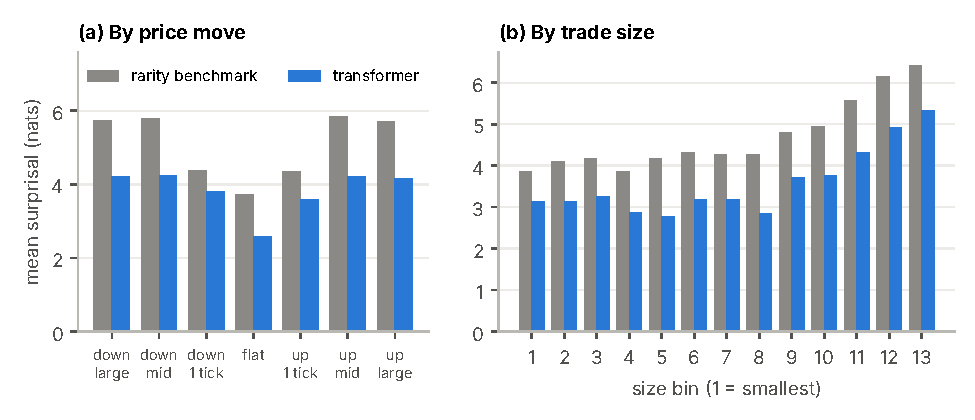
\includegraphics[width=\linewidth]{figures/classes.pdf}
\caption{Mean surprisal on the test month by (a) price-move class and (b) size bin, for the rarity benchmark and the transformer.}
\label{fig:classes}
\end{figure}

%% ------------------------------------------------------------------------------------
\section{Reproducibility}\label{app:repro}

The whole study runs from one script, \texttt{python run.py}.
It performs these steps in order.
\begin{enumerate}
  \item Download and verify the data.
  \item Build events and tokens.
  \item Train the three seeds and select one.
  \item Score the test month, evaluate, and export the weights.
\end{enumerate}
It writes a checkpoint every 10 minutes of wall time, so that an interrupted run can resume, and it prints a status line with an estimated time to completion every minute.
On a laptop with a four-core Intel i5-1038NG7 CPU and no GPU, a full run takes about six hours of computation.
Each seed trains for about \TrainMinutes{} minutes and the scoring takes about two hours.

The weights of the selected seed, the fitted tokeniser and a small file of prompt excerpts are in the repository, with a local interface for generating continuations of a tape.
The figures, numbers and tables of this paper are produced from the run outputs by \texttt{paper/make\_figures.py}.
The text quotes numbers only through the generated files, so the paper cannot disagree with the run.
The rarity benchmark and the other descriptive checks of \cref{app:rarity} are computed in that script.

\end{document}
